\chapter{Design and Implementation}

% - Should the subsections more or less reflect the columns in the table?

\section{Hardware Design}

% - EXPLAIN MORE ABOUT HARDWARE CHOISES, why these specific componens. What were the requirements for choosing these components

The first step was to evaluate what components are required for the robot to have basic navigation capabilities.
Commercially available low power components have been evaluated, where the main criteria was a low minimal supply voltage.
This section will explain each part of the robot in more detail and a complete overview of the robot is shown in Figure \ref{fig:robot_overview}.

\vspace{1em}
\begin{figure}[h!]
	\centering
	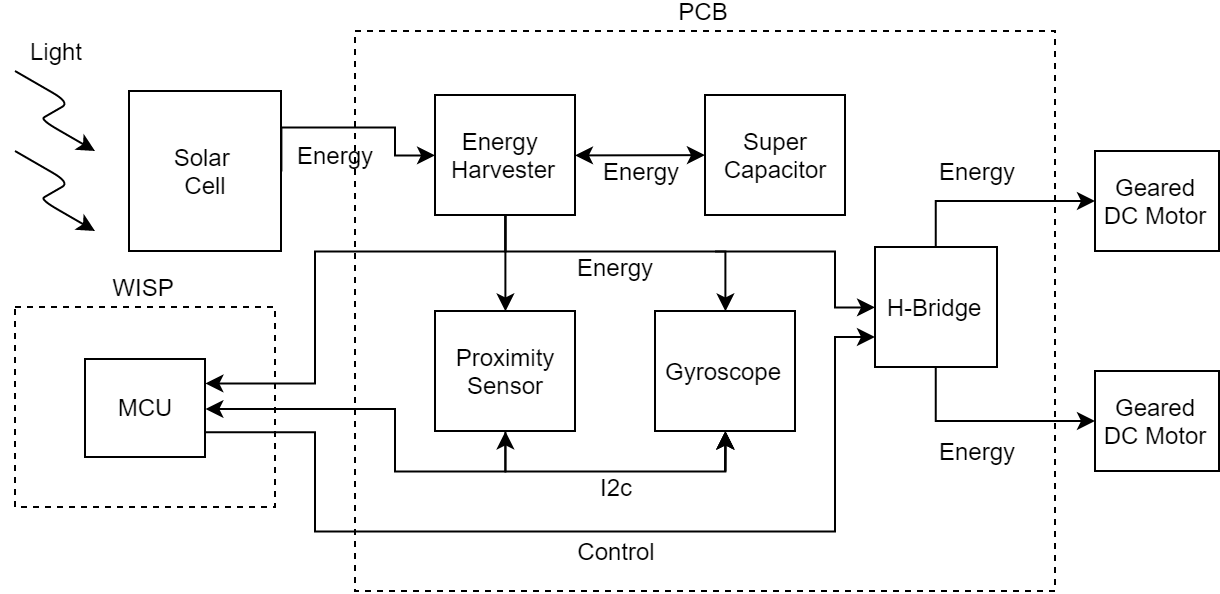
\includegraphics[width=\textwidth]{pics/schematic_robot_v2.png}
	\caption{Schematic overview of the robot.}
	\label{fig:robot_overview}
\end{figure}

\subsection{Energy Source}
%TODO refer to preliminaries section
Solar energy is harvested from two IXYS SLMD121H04L-ND solar cells~\cite{ixolar_slmd121h04l_2017} in parallel.
These monocrystalline solar cells have a high efficiency of 22\%, allowing energy harvesting even in low light conditions.
The solar cells are connected to a energy harvester. 

\subsection{Energy Harvesting and Storage}
\label{sec:imp_energy_harvesting}
Energy is harvested using a Texas Instruments BQ25570 energy harvester~\cite{bq25570_2017}, which includes a nanopower boost charger with maximum power point tracking to extract the optimal amount of energy. 
The harvested energy is stored in a 22\,mF - 4.5\,V supercapacitor from AVX~\cite{avx_bestcap_2017}, chosen for its low leakage current and small size.
The Texas Instruments BQ25570 has a buck converter to efficiently regulate the capacitor voltage down to the system voltage.

The minimal supply voltage is determined by the component with the highest minimal voltage requirement, in this case 2.0\,V.
To make sure that a small drop in system voltage would not create instability a margin of 0.2\,V was added, resulting of a system voltage of 2.2\,V.
External resistors can be used to program voltage thresholds, allowing to automatically enable and disable the buck converter based on minimum and maximum thresholds.
Additionally the resistors are used to set the overvoltage protection and the buck converter output voltage.

\subsection{Computation}
\label{sec:imp_computation}

The robot is designed around a WISP 5 \cite{wisp5_wiki_2017}, a battery-free platform for low power sensing, computation and communication.
This platform has the ability to communicate with RFID readers and is powered by the carrier signal emitted by the reader.
However, the communication range and the power that can be harvested is limited.
Therefore communication is currently not implemented and a different energy source for harvesting will be used as described in Section \ref{sec:energy_harvesting}.
Currently only the MCU from the WISP is being utilized: a Texas Instruments MSP430FR5969 ultra low power microcontroller.
This MCU can operate at 16\,MHz and features 64\,KB FRAM, 2\,KB SRAM and 40 IO-ports \cite{msp430fr5969_2017}.

\subsection{Sensing}
\label{sec:imp_sensing}

The robot has access to basic sensors which can be interfaced trough I2C.
For detecting obstacles in front of the robot, a Maxim Integrated MAX44000 proximity sensor was added of the robot facing forward.
This sensor switches a IR led at high frequency to reduce the power consumed.
The same sensor is based around a photo-diode it can be used to measure the amount of ambient light as well.
To allow for controlled movements the robot has a Bosch Sensortec BMG250 low power triaxial gyroscope to measure yaw-rate, used to correct it's heading when necessary.

\subsection{Locomotion}

% tell that also higher geared motors were tried??

Two 25:1 sub-micro plastic planetary gearmotors from Precision Microdrives~\cite{gearmotor_206-110_2017} are mounted in a 3D printed frame.
The motors are positioned diagonally opposite from each other making the robot as compact as possible, while this differential drive configuration allows the robot to steer.
Small plastic wheels with rubber tires are mounted directly on each of the motor shafts.
Behind these two motors a free running caster wheel is mounted to the frame, acting as a third support point for the robot.

\subsection{Motor Control}
\label{sec:imp_motor_control}

The speed (and the current consumption) of each motor can be controlled individually using Pulse-Width-Modulation (PWM).
The MCU can use the H-bridge to enable, disable and control the direction of rotation of each individual motor.
Typically MCU IO-ports are limited in the amount of current that they can supply.
MOSFETs inside a Texas Instruments DRV8836 dual H-bridge~\cite{drv8836_2017} allow efficient regulation of larger currents to the motors.

\subsection{Integration}

%TODO add photograph of complete robot here!
Now that all the parts have been chosen, they can be connected together to form the robot.
A Printed Circuit Board (PCB) has been designed using EAGLE PCB design and schematic software.
For the reason of increased stability, ease of connection, reduction of the total weight of the robot and was required because of the small size ICs (no lead packaging).
A detailed schematic of the PCB can be found in Appendix \ref{app:schematic_robot}.

Most components are part of the PCB only the larger components are mounted externally, the solar panel, WISP and the motors.
The PCB contains headers to connect the solar panel, a header to connect all the required pins from the WISP and a additional header to connect a battery for testing purposes.
Most reference designs are extendable but this adds complexity, while weight and size are the main constraints in this robot design.
A overview of both the top and bottom side of the PCB is shown in Figure \ref{fig:pcb_robot}.

% Features of the pcb, wisp regulator allows powering from battery for testing

%The top of the PCB contains all the surface mount components that are soldered to the PCB using a reflow oven. 
%When the boards come out of the oven, the headers, motors and supercapacitor are soldered to the boards by hand.

\begin{figure}[h!]
	\centering
	\begin{subfigure}[b]{0.45\textwidth}
		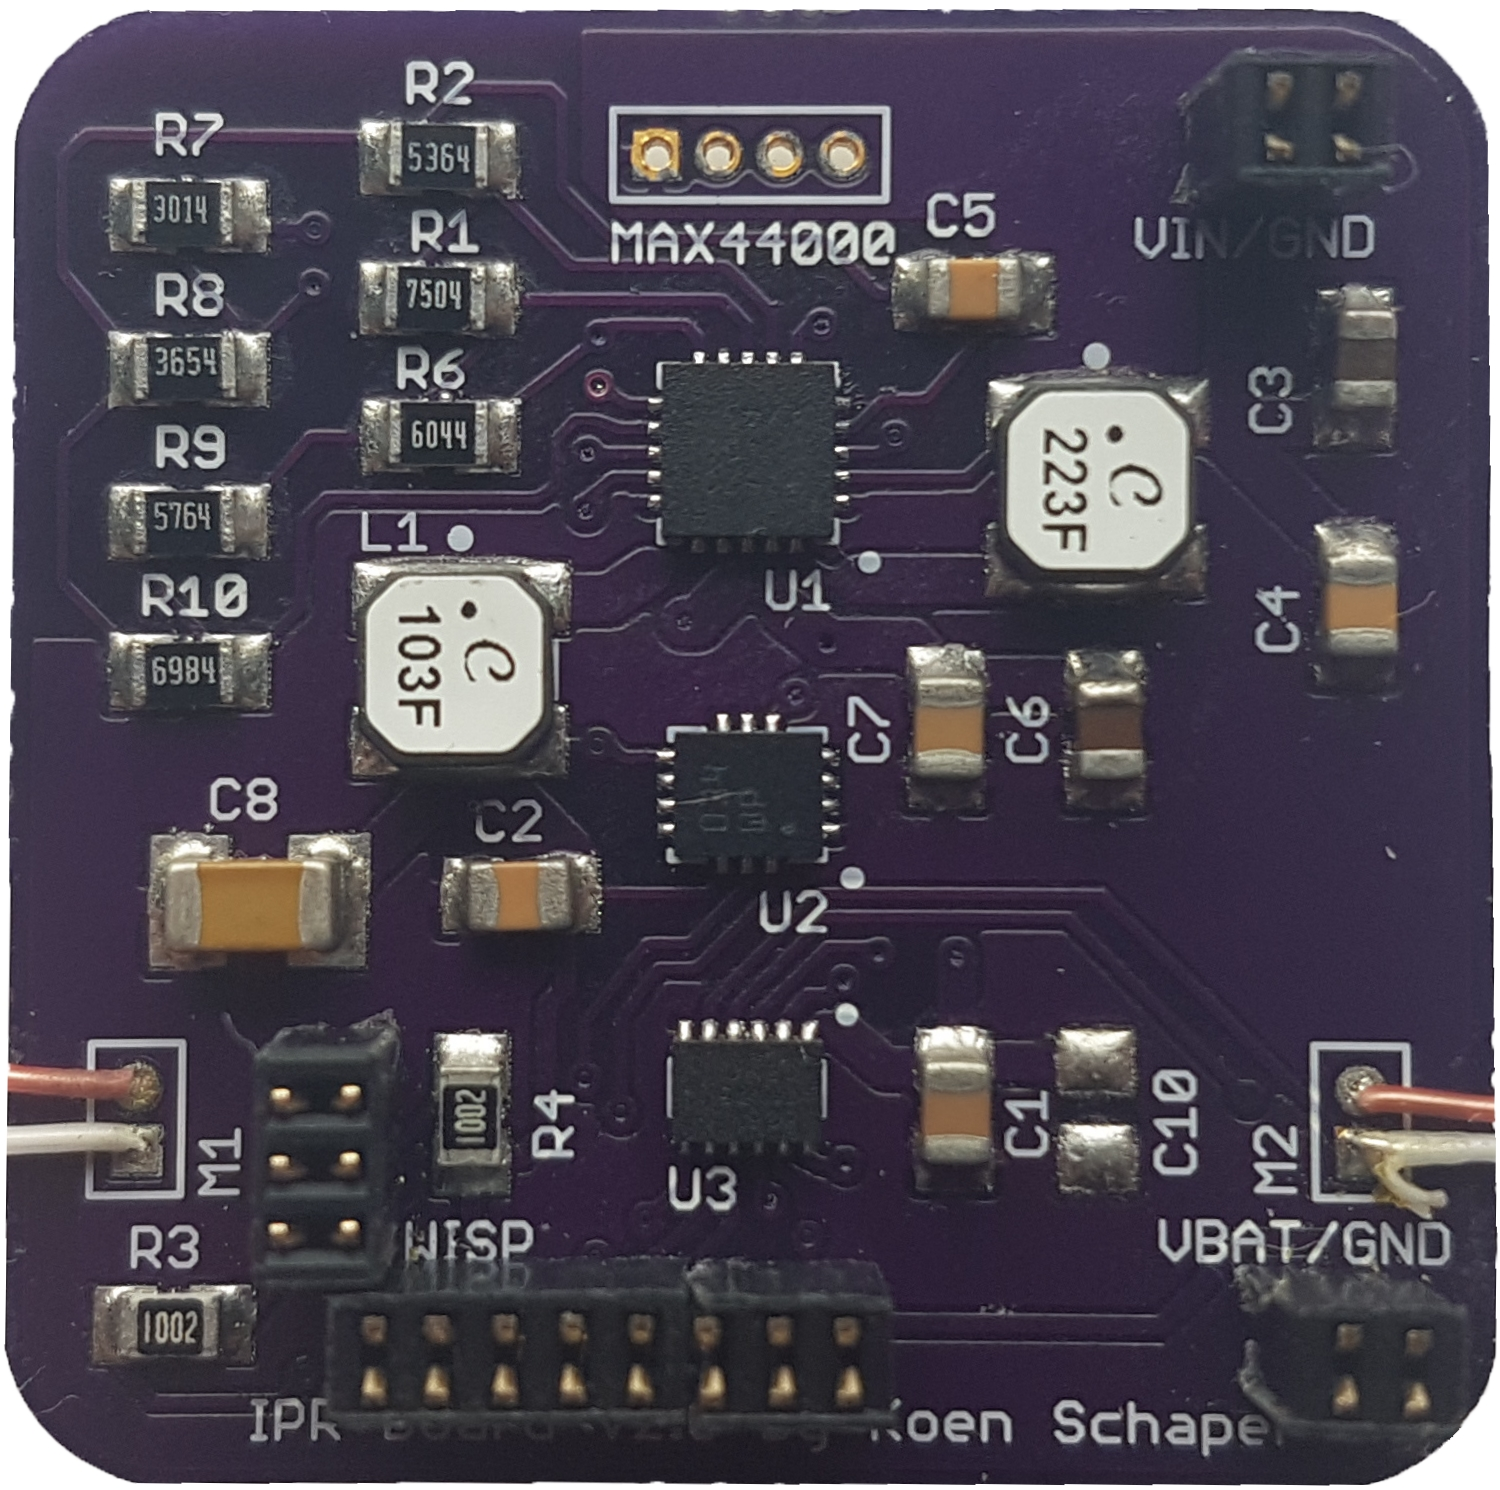
\includegraphics[width=\textwidth]{pics/pcb_front.jpg}
		\caption{Top side of the PCB}
		\label{fig:pcb_robot_front}
	\end{subfigure}
	\qquad
	\begin{subfigure}[b]{0.45\textwidth}
		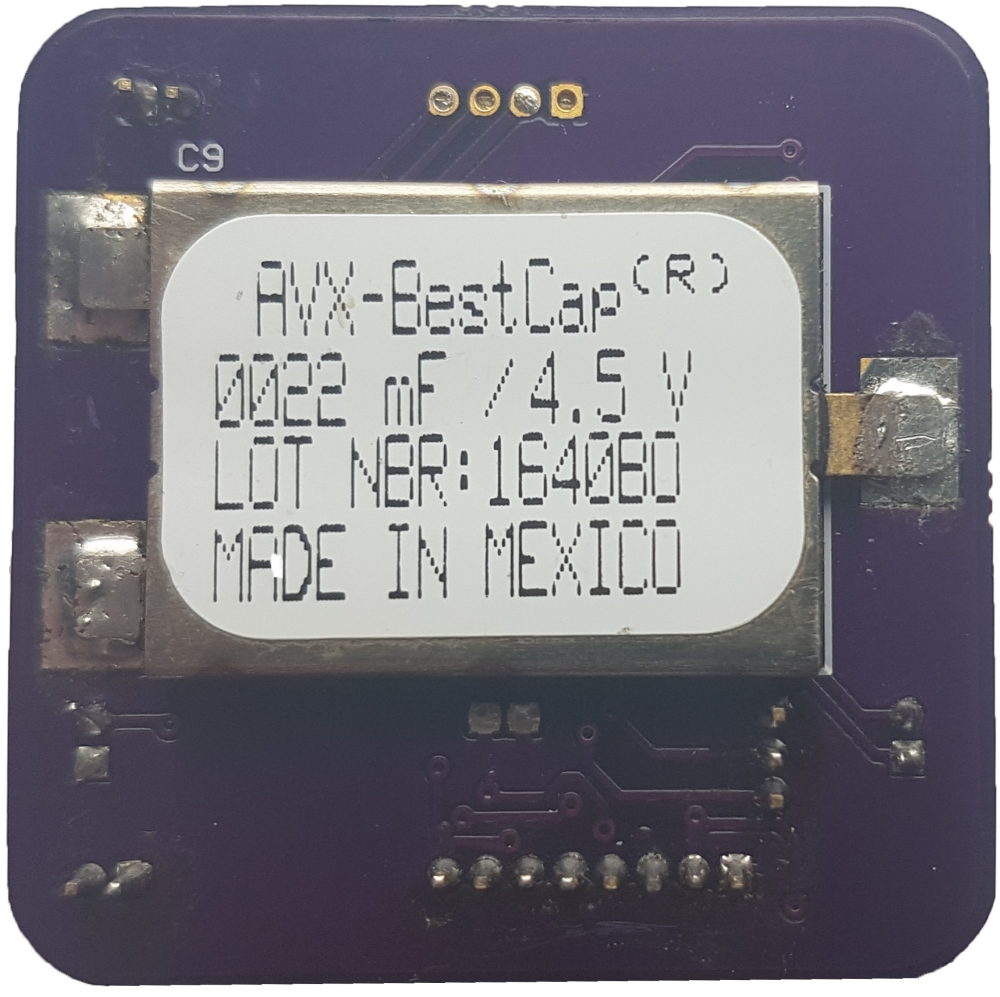
\includegraphics[width=\textwidth]{pics/pcb_back.jpg}
		\caption{Bottom side of the PCB}
		\label{fig:pcb_robot_back}
	\end{subfigure}
	\caption{The PCB designed for the robot}
	\label{fig:pcb_robot}
\end{figure}

\subsection{Energy Expenditure}

The average current consumed of each component was measured with a Monsoon Power Monitor \cite{monsoon_powermonitor_2017}.
The measurement was preformed as follows, first a two second current trace was recorded of the current consumed by the MCU on the WISP.
The MCU was then used to enable each component individually, followed by a two second current measurement with the enabled component.
The average of each current trace was calculated, and the current consumed by the microcontroller subtracted from the current consumed by each component.
The measurement result is provided in Table \ref{tab:avg_cur_comp}.

% Make a overview of the cost to build a robot

\begin{table}[t]
	\centering
	\begin{threeparttable}
		\caption{Average consumed current for each individual component at 2.2 V.}
		\label{tab:avg_cur_comp}
		\begin{tabular}{|l|l|} 
			\hline
			Part & Active Current \\
			\hline\hline
			Proximity sensor & 119 \textmu A \\
			Gyroscope & 848 \textmu A\\	
			Microcontroller @ 8MHz & 522 \textmu A\\
			H-bridge & 349 \textmu A \\
			Two DC motors\textsuperscript{1} & 27--50 mA  \\
			\hline \hline
			Total & 29--52 mA \\
			\hline
		\end{tabular}
		\begin{tablenotes}
		\small
		\item [1] Current consumed varies per motor and motor speed
		\end{tablenotes}
	\end{threeparttable}
\end{table}

\subsection{Cost}

By using off-the-shelf components that that are readily available allows to build multiples of this robot with ease.
Keeping the cost down per individual is important when these robots are used in collectives.
Table \ref{tab:cost_robot} shows the total price to build a single robot, assuming a minimal fabrication quantity of 20.
This overview is compiled by querying the component prices of different suppliers, Farnell, Digikey, Mouser, Pololu, and OshPark.
The price for the PCB does not include the price of assembling the PCB, as this is currently done by hand.
Secondly, the cost of a WISP / MCU is currently not included in the price.
From this table can be concluded that the cost of building a transiently powered robot is comparable to the cost of other reference small robotic platforms.


\begin{table}[t]
	\centering
	\caption{Cost per robot}
	\label{tab:cost_robot}
	\begin{tabular}{|l|l|} 
		\hline
		Part & \euro Price \\
		\hline\hline
		Solar panel & 9,60\\
		Supercapacitor & 7,43\\
		Harvester & 5,48 \\
		Proximity sensor & 3,98 \\
		Gyroscope & 2,81\\	
		H-bridge & 1,47 \\
		Two DC motors & 18,51 \\
		Wheels & 3,08\\
		PCB & 2,50 \\
		Passive SMD & 4,53\\
		\hline \hline
		Total & 59,39 \\
		\hline
	\end{tabular}
\end{table}


\section{Control Design}

\section{Software Implementation}

\subsection{Calibration of the Motors}
\label{sec:calib_motors}

%TODO STIL VALID? (Write about why valid to assume a constant speed on a single surface)
The motors used for robots are powered directly from the battery as linear or switch-mode power regulators are not able to supply the high start-up currents.
When the motors are powered from the battery the supplied voltages drops while energy is consumed for the battery.
Since the speed of the motor is dependent on the supply voltage the speed of the motor will also decrease while energy is consumed from the battery.
However, the use of a supercapacitor requires a regulator to make efficient use of the energy stored, as described in Section \ref{sec:imp_energy_harvesting}.
A benefit of keeping the supply voltage constant is that voltage is eliminated as a factor in determining the motor speed.
By making the assumption that the robot will only travel on a flat surface, the steady state speed is considered ``constant" given a certain PWM duty cycle.


\subsubsection{PWM Frequency for Linear Motion Control}
% Write about linear motion control dc motor vs pwm
% Reference: https://www.precisionmicrodrives.com/application-notes/ab-022-pwm-frequency-for-linear-motion-control

Pulse width modulation (PWM) is used to control the speed of the motors, the average current supplied to the motors can be regulated by changing the duty cycle.
When the motor is at rest its equivalent circuit consists of a resistance and inductance in series.
When voltage is applied to the motor the rate at which the current rises is limited by the inductance. 
All RL circuits have a time constant: $\tau = L / R$ and the current reaches its maximum steady state at $5\tau$. 
The motors used for the robot have a typical resistance R of 14.5\,$\Omega$ and an inductance of L = 70\,$\mu$H~\cite{gearmotor_206-110_2017}.
Therefore the minimum pulse width should be equal to:

\begin{equation}
	5\tau_{\min} = 5 \frac{L}{R} 
\end{equation}

From this can be calculated that the minimum pulse width should be $5\tau = 5 \cdot \frac{70 \cdot 10^{-6}}{14.5} = 24.14\,\mu s$.
If a minimum pulse width of is assumed, than the maximum PWM frequency becomes:

\begin{equation}
	f_{\max} = \frac{t_{\text{on}}}{5\tau}\cdot 100
\end{equation}

If the PWM frequency is assumed to be at least 5\% than the maximum PWM frequency is equal to $\frac{5}{24.14 \cdot 100} = 2071.25\,Hz$.
The PWM frequency will be set to 2\,kHz and later will be verified that the duty cycle will never go below the minimum of 5\%.

% -Write how the pwm control signals are generated for the H-bridge. 
The PWM signals are generated by the microcontroller on the WISP.
Four IO-ports are available on the WISP which can be directly controlled by a single timer.
The timer is configured to use a compare register for each of the ports.
When the timer reaches a value that corresponds to a value one of the compare registers the connected port is toggled automatically.
This way the overhead is minimized because no interrupt service routine is required.

\subsubsection{Minimal Duty Cycle}

The minimal PWM duty cycle to produce a torque that is able to overcome the static friction between the wheels and a surface the robot is moving on.
Each motor is physically different and the friction in the gearbox can variate as well, which results in a variating output speeds per motor.
Since the robot uses two motors in differential drive configuration, a minimum PWM duty cycle has to be found for each motor.
This is accomplished by setting a PWM duty cycle at which both motors are rotating and slowly backing down the PWM duty cycle until one or both stop turning.
The minimum PWM duty cycle, allowing the wheels to rotate, is stored as a calibration and added to every motor set point.
If the robot is set to run at the minimum speed does not mean that the motors run at the same speed.

\subsubsection{Maximal Duty Cycle}
% -Write about maximum speed due to enabling two motors and their startup current peak! show figure!!
% Does more gearing (more torque) reduce the current peak??

The maximum PWM duty cycle is bounded by the amount of current that the buck converter and bulk capacitor can supply.
The back electromotive force (back EMF) of a DC motor at rest is equal to zero.
%TODO ADD ref for above statement
When voltage is applied to the motor, current rises as quickly as the inductance in the motor windings allows. 
The current peaks when the rotor starts to rotate and a back EMF is generated.
The back EMF will further increase while the motor accelerates to its steady state speed, and the speed is limited by the voltage supplied.
Lowering the PWM duty cycle reduces both the maximum current peak and the steady state current and therefore can be used to reduce the motor start current demand.
The maximum PWM duty cycle can be found by increasing the duty cycle until the robot is not able to start a movement from that PWM set point. 

\subsection{Closed loop feedback for controlled movements}

%The robot uses two physically different motors in differential drive configuration which are mounted in a non-symmetrical way.
Open loop movement using just a calibrated motor values has been used in previous work \cite{legoc_uist_2016}, but it can be time consuming and any little disturbance will trow the robot off course.
The gyroscope is used to obtain the current yaw-rate and correct the robots heading.
Controlled movements are possible using closed loop feedback, where the heading is used to update the motor control values.

The robot can be controlled using three different commands, one for straight trajectories, one for left and one for right turns.
When a command is executed a control loop will run until the provided target is reached.
A timer running periodically calling an interrupt service routine which executes the control loop.   
Each command requires different initial values, set points and tuning parameters, these are set accordingly before the control loop is enabled.

\subsubsection{Controlled straight trajectories}

% -Why pid for straight movements and not a simple p controller?
% --Fast reaction on disturbances without osccilation??
%TODO -Write about bounding the pid output, because otherwise the motors of the robot could stall, if the motor setpoint is to high

The control loop for straight trajectories obtains the yaw-rate from the gyroscope and uses this as an input for the Proportional Integral Derivative (PID) controller.
The PID will continuously try to force the yaw-rate to zero for a given target motor speed.
% $ e(t) = 0 - yaw(t)$
Using the output of the PID controller the target motor speed of each motor is adjusted in opposite direction.
The loop will stop automatically when the required target is reached.
%TODO Explain that the target distance is with a calibrated value.

\begin{equation}
\text{output}(t) = K_{p}e(t) + K_{i} \int_{0}^{t}e(\tau)d\tau + Kd\frac{d}{dt}e(t) \qquad [\text{rad/s}]
\end{equation}

\subsubsection{PID tuning using Ziegler-Nichols method}

%TODO -Write about tuning the pid controller using Ziegler–Nichols tuning method (method 2), closed loop, Critical gain.

A PID loop can be tuned using three different tunable gains ($K_{p}$, $K_{i}$, $K_{d}$).
Tuning can be done trough a trail and error approach but a faster way of tuning is to use the Zigeler-Nicholos method.
It starts with increasing or decreasing $K_{p}$ until constant oscillation occurs.
From Figure \ref{fig:ultimate_gain} can be seen how the proportional gain was increased until eventually the robot started to oscillate.
With a proportional gain of 0.13 the robot starts light oscillation at the end, but this is not always the case and can be a result of the surface the robot was driving on.
% Tell something about how the right values are determined
To reduce the oscillation a $T_{u}$ of 0.2 was added as can be determined from Figure \ref{fig:gain_tuning}.
From this figure can be seen that the robot is more stable and does not have the tendency to oscillate anymore.
%Robots was driving on surface that was not super flat, therefore the gyro signal is noisy.
The tuning process was speeded up by setting the minimum motor duty cycle as it made the robot a lot more responsive, this was described earlier in Section \ref{sec:calib_motors}.

%TODO -Add figure with critcial gain + mark period Tu

\begin{figure}
	\begin{subfigure}[b]{0.49\textwidth}
		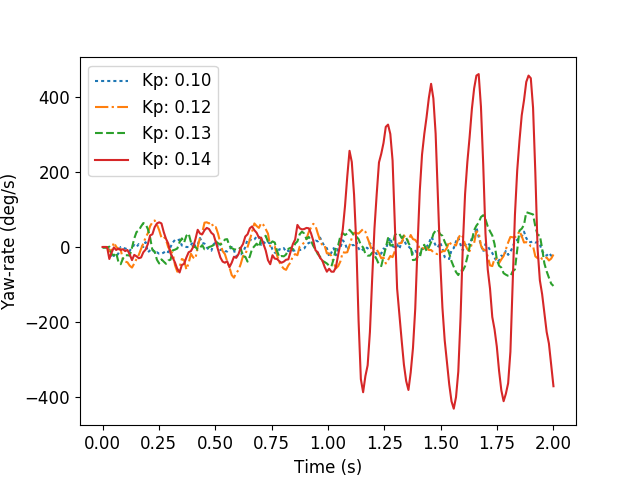
\includegraphics[width=\textwidth]{pics/straight_ku.png}
		\caption{Increase $K_p$ until constant oscillation}
		\label{fig:ultimate_gain}
	\end{subfigure}
	\begin{subfigure}[b]{0.49\textwidth}
		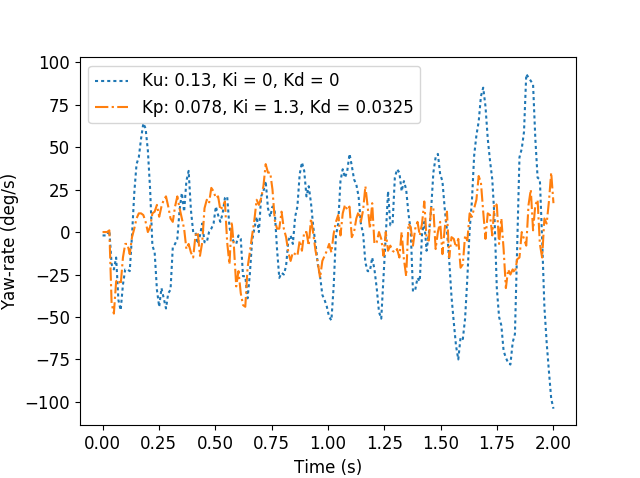
\includegraphics[width=\textwidth]{pics/straight_ku_with_tu.png}
		\caption{Find the constant oscillation period}
		\label{fig:gain_tuning}
	\end{subfigure}
	\caption{Tuning the PID controller using the ultimate gain method.}
\end{figure}

\subsubsection{Controlled curved movements} 

The same PID control loop can be used to command the robot to make curved movements.
Instead of an angular velocity set point of zero, an turn rate needs to be specified.
This desired angular velocity can be a determined from the radius of the circle that the robot needs to turn and the calibrated target speed.
By integrating the angular velocity an angle estimate is obtained, which is used to verify if the angle target given is reached within two degrees.
In case this is true the loop will exit automatically.

\subsubsection{Controlled turns}

The control loop for controlled turning uses the angle, which is obtained by integrating the yaw-rate sensor data from the gyroscope.
A P controller is used to rotate the robot to the desired angle, the proportional gain is directly influencing turn speed of the robot.
The motor control values are set to run the motors opposite directions and are equal to the output of the P controller.
These values will keep decreasing until the robot rotates to the desired angle.
The set point is assumed to be reached when the angle is within two degrees of the target, in this case the loop will stop automatically.
To allow enough precision to measure if the target is within these two degrees, the timer which executes the control loop was set to run at 100\,Hz.
Secondly, the proportional gain should not be set to low because the robot might not able to reach the target but also not to high as it can overshoot the target.

\subsection{Persistent movement}

Normally when a robot is battery powered, it can execute some predefined movements and stop when required.
In case of the transiently powered robot one movement or a series of movements is likely to require multiple power cycles to complete.
To be able to finish a movement and not reset i.e. redo the same movement, a simple check pointing method is used to keep the program state across power cycles.
A persistent counter registers the progress in the set of movements.
In the control loop only the progress in moving towards a set point is stored in non-volatile FRAM memory, which depending on the movement can be a required time or angle.
The right and left motor speed which are tuned by the controllers are not saved and restored after a power interrupt.
The motors have a startup phase the controller needs to react differently compared to the steady state, constant speed movement of the robot. 